\documentclass[paper=a4,margin, fontsize=11pt]{scrartcl} % A4 paper and 11pt font size
\usepackage[T1]{fontenc} % Use 8-bit encoding that has 256 glyphs
%\usepackage{fourier} % Use the Adobe Utopia font for the document - comment this line to return to the LaTeX default
\usepackage{pdfpages}
\usepackage[english]{babel} % English language/hyphenation
\usepackage{amsmath,amsfonts,amsthm} % Math packages
%\usepackage{sectsty} % Allows customizing section commands
\usepackage{blindtext}
\usepackage[utf8]{inputenc}
\usepackage{graphicx}
\graphicspath{{Pictures/}}
%\allsectionsfont{\left\normalfont\scshape} % Make all sections centered, the default font and small caps
%\usepackage{fancyhdr} % Custom headers and footers
%\pagestyle{fancyplain} % Makes all pages in the document conform to the custom headers and footers
%\fancyhead{} % No page header - if you want one, create it in the same way as the footers below
%\fancyfoot[L]{} % Empty left footer
%\fancyfoot[C]{\thepage} % put page number in center footer
%\fancyfoot[C]{} % Empty right footer
%\renewcommand{\headrulewidth}{0pt} % Remove header underlines
%\renewcommand{\footrulewidth}{0pt} % Remove footer underlines
\setlength{\headheight}{0pt} % Customize the height of the header

\numberwithin{equation}{section} % Number equations within sections (i.e. 1.1, 1.2, 2.1, 2.2 instead of 1, 2, 3, 4)
\numberwithin{figure}{section} % Number figures within sections (i.e. 1.1, 1.2, 2.1, 2.2 instead of 1, 2, 3, 4)
\numberwithin{table}{section} % Number tables within sections (i.e. 1.1, 1.2, 2.1, 2.2 instead of 1, 2, 3, 4)

\setlength\parindent{0pt} % Removes all indentation from paragraphs - comment this line for an assignment with lots of text

%----------------------------------------------------------------------------------------
%	TITLE SECTION
%----------------------------------------------------------------------------------------
\title{	
\normalfont \normalsize 
\textsc{EENG 517}\\ 
\huge Midterm \\ % The assignment title
}

\author{Dana Martin} % Your name

\date{\normalsize Due: 03/10/16}

\begin{document}

\maketitle % Print the title


\section*{Problem 1 (15 points)}
Consider the following system:

\begin{align*}
\ddot{y_1}+4\dot{y_1}+3y_1+\ddot{y_2}+3\dot{y_2}+2y_2=u_1\\
\ddot{y_1}+5\dot{y_1}+6y_1+\ddot{y_2}+5\dot{y_2}+6y_2=u_2\\
\end{align*}

\subsection*{a. Give a matrix fraction description of the system}
Assume initial conditions to be zero... taking the Laplace Transform, we find,
\begin{align}
s^2Y_1(s)+4sY_1(s)+3Y_1(s)+s^2Y_2(s)+3sY_2(s)+2Y_2(s)=U_1(s)\\
s^2Y_1(s)+5sY_1(s)+6Y_1(s)+s^2Y_2(S)+5sY_2(s)+6Y_2(s)=U_2(s)
\end{align}

\begin{align*}	
\begin{bmatrix}s^2+4s+3 && s^2+3s+2 \\ s^2+5s+6 && s^2+5s+6 \end{bmatrix} \begin{bmatrix}Y_1(s) \\ Y_2(s) \end{bmatrix} = \begin{bmatrix} U_1(s) \\ U_2(s)\end{bmatrix}
\end{align*}

$D(s)Y(s)=N(s)U(s)\rightarrow Y(s)=D(s)^{-1}N(s)U(s)$ where $G(s)=D(s)^{-1}N(s)$

\begin{align}
	\begin{bmatrix}
		Y_1(s)\\Y_2(s)
	\end{bmatrix}
	= \begin{bmatrix}s^2+4s+3 && s^2+3s+2\\ s^2+5s+6 && s^2+5s+6 \end{bmatrix}^{-1}\begin{bmatrix}1 && 0\\0 &&1\end{bmatrix}\begin{bmatrix}U_1(s)\\U_2(s)\end{bmatrix}
\end{align}\\

Equation 0.3 is the matrix fraction description of the system.

\subsection*{b. Give a transfer matrix description of the system}

From above we know that $G(s)=D(s)^{-1}N(s)$

\begin{align*}
D(s)^{-1}=&\frac{1}{(s^2+4s+3)(s^2+5s+6)-(s^2+3s+2)(s^2+5s+6)}
\begin{bmatrix}(s+2)(s+3) && -(s+1)(s+2)\\ -(s+2)(s+3) && (s+1)(s+3)\end{bmatrix}\\
=&\frac{1}{(s+1)(s+3)(s+2)(s+3)-(s+1)(s+2)(s+2)(s+3)}
\begin{bmatrix}(s+2)(s+3) && -(s+1)(s+2)\\ -(s+2)(s+3) && (s+1)(s+3)\end{bmatrix}\\
\newline
=&\begin{bmatrix}
\frac{1}{(s+1)(s+3)-(s+1)(s+2)} && \frac{-1}{(s+3)(s+3)-(s+2)(s+3)}\\
\frac{-1}{(s+1)(s+3)-(s+1)(s+2)} && \frac{1}{(s+2)(s+3)-(s+2)(s+2)}
\end{bmatrix}
\end{align*}

\begin{align*}
D(s)^{-1}N(s)=\begin{bmatrix}
\frac{1}{(s+1)(s+3)-(s+1)(s+2)} && \frac{-1}{(s+3)(s+3)-(s+2)(s+3)}\\\frac{-1}{(s+1)(s+3)-(s+1)(s+2)} && \frac{1}{(s+2)(s+3)-(s+2)(s+2)}
\end{bmatrix} \begin{bmatrix}1 && 0\\ 0 && 1\end{bmatrix}
\end{align*}

\begin{align}
	G(s)= \begin{bmatrix} \frac{1}{(s+1)(s+3)-(s+1)(s+2)} && \frac{-1}{(s+3)(s+3)-(s+2)(s+3)} \\ \frac{1}{(s+1)(s+3)-(s+1)(s+2)} && \frac{1}{(s+2)(s+3)-(s+2)(s+2)}\end{bmatrix}
\end{align}

Equation 0.4 is the transfer matrix description of the system

\section*{Problem 2 (10 points)}
For the following system, find its transfer matrix:

\begin{align*}
\dot{x}=&\begin{bmatrix} -1 && 1 \\ 0 && -2\end{bmatrix}x
+\begin{bmatrix}1 && 4\\1 && 1\end{bmatrix}\\
y=&\begin{bmatrix}2 && 0\\0 && 1\end{bmatrix}x
\end{align*}

The transfer matrix of a state-space system is given by $G(s)=C(sI-A)^{-1}B$.

\begin{align*}
sI-A=\begin{bmatrix}s && 0 \\0 && s\end{bmatrix} -
\begin{bmatrix} -1 && 1\\ 0 && -2\end{bmatrix}=\begin{bmatrix} s+1 && -1 \\0 && s+2\end{bmatrix}\\
\end{align*}

\begin{align*}
(sI-A)^{-1} = \frac{1}{(s+1)(s+2)-(-1)(0)}\begin{bmatrix}s+2 && 1\\0 && s+1\end{bmatrix}=\begin{bmatrix}
\frac{s+2}{(s+1)(s+2)+1} && \frac{1}{(s+1)(s+2)+1} \\ 0 && \frac{s+1}{(s+1)(s+2)+1}\end{bmatrix}
\end{align*}

\begin{align*}
C(sI-A)^{-1}=&\begin{bmatrix}2 && 0 \\ 0 && 1\end{bmatrix}\begin{bmatrix}\frac{s+2}{(s+1)(s+2)+1} && \frac{1}{(s+1)(s+2)+1} \\ 0 &&\frac{s+1}{(s+1)(s+2)+1}\end{bmatrix}\\
=&\begin{bmatrix}\frac{2s+4}{(s+1)(s+2)+1} && \frac{2}{(s+1)(s+2)+1} \\ 0 && \frac{s+1}{(s+1)(s+2)+1}\end{bmatrix}
\end{align*}

\begin{align*}
C(sI-A)^{-1}B=&\begin{bmatrix}
\frac{2s+4}{(s+1)(s+2)+1} && \frac{2}{(s+1)(s+2)+1}\\ 0 && \frac{s+1}{(s+1)(s+2)+1}\end{bmatrix}\begin{bmatrix} 1 && 4 \\ 1 && 1\end{bmatrix}\\
=&\begin{bmatrix}
\frac{2s+4}{(s+1)(s+2)+1}+\frac{2}{(s+1)(s+2)+1} && \frac{8s+16}{(s+1)(s+2)+1}+\frac{2}{(s+1)(s+2)+1} \\ \frac{s+1}{(s+1)(s+2)+1} && \frac{s+1}{(s+1)(s+2)+1}\end{bmatrix}
\end{align*}

\begin{align*}
\boldsymbol{G(s)=\begin{bmatrix}
\frac{2s+6}{(s+1)(s+2)+1} && \frac{8s+18}{(s+1)(s+2)+1} \\ \frac{s+1}{(s+1)(s+2)+1} && \frac{s+1}{(s+1)(s+2)+1}\end{bmatrix}}
\end{align*}

\section*{Problem 3 (10 points)}
Consider the following SISO unstable first order-system:
\begin{align*}
\dot{x}=&3x+u\\
y=&5x
\end{align*}
For this system design a state feedback control law (u=kx+r) to place the closed-loop pole(s) at s=-1.\\
\\
For a SISO closed loop system, the transfer function is $\frac{Y}{R}=\frac{GC}{1+GC}\rightarrow\frac{n_cn_g}{d_cd_g+n_cn_g}$\\
\\
\begin{center}
For the plant $G=\frac{5}{s-3}$\\
For the controller $C=\frac{r}{s-k}$
\end{center}
Rearranging the top equations into the form given by the closed loop transfer function the resulting equation is:

\begin{align*}
\frac{5r}{(s-3)(s-k)+5r}
\end{align*}
Setting r=1, the denominator of the transfer function becomes
$s^2-ks-3k+5$. Since we want the closed loop poles of the system to reside at s=-1, we need the denominator to factor into (s+1)(s+1).  Knowing this, we can set up an equation to solve for the value of the coefficient k.
\begin{align*}
-ks-3k+5=2s+1\\
-k-3k+5=3\\
-4k+5=3 \rightarrow \boldsymbol{k=\frac{1}{2}}
\end{align*}
With the values for r and k known the control law becomes:
\begin{align*}
\boldsymbol{u=\frac{1}{2}x+1}
\end{align*}
\section*{Problem 4 (15 points)}
Give ccf and diagonal realizations of the following system (be careful to divide out any D-matrix terms):

\begin{align*}
H(s)=\begin{bmatrix}\frac{2}{s+1} && \frac{2s-3}{(s+1)(s+2)}\\\frac{s-2}{s+1} && \frac{s}{s+2}\end{bmatrix}
\end{align*}

Simplifying the above matrix through algebraic long division the resulting matrices are:\\

\begin{align*}
\hat{H}(s)=&\begin{bmatrix}
\frac{2}{s+1} && \frac{2s-3}{(s+1)(s+2)} \\ \frac{-3}{s+1} && \frac{2}{s+2}\end{bmatrix}\\
D=&\begin{bmatrix} 0 && 0 \\ 1 && 1 \end{bmatrix}
\end{align*}

For ccf form, a common denominator must be factored out.\\

\begin{align*}
\frac{1}{(s+1)(s+2)}\begin{bmatrix}2(s+2) && 2s-3 \\ -3(s+2) && 2(s+1)\end{bmatrix}\\
\\
=\frac{1}{(s+1)(s+2)}\begin{Bmatrix}s\begin{bmatrix} 2 && 2\\-3 && 2\end{bmatrix} + \begin{bmatrix}4 && -3 \\ -6 && 2\end{bmatrix} \end{Bmatrix}
\end{align*}

The Controller Canonical Form Realization of the given system is described by the matrices:

\begin{align*}
A&=\begin{Bmatrix}-3&\begin{bmatrix}1 && 0\\ 0 && 1 \end{bmatrix} && -2&\begin{bmatrix}1 && 0\\0 && 1\end{bmatrix}\\&\begin{bmatrix}1 && 0\\0 &&1\end{bmatrix} && &\begin{bmatrix}0 && 0\\ 0 && 0\end{bmatrix}\end{Bmatrix}\\
B&=\begin{Bmatrix}
\begin{bmatrix}1 && 0\\0 && 1\end{bmatrix}\\\begin{bmatrix}0 && 0\\0 && 0\end{bmatrix}\end{Bmatrix}\\
C&=\begin{Bmatrix}
\begin{bmatrix}2 && 2\\-3 && 2\end{bmatrix} && \begin{bmatrix}4 && -3\\-6 && 2\end{bmatrix}\end{Bmatrix}\\
D&=\begin{Bmatrix}0 && 0\\1 && 1\end{Bmatrix}
\end{align*}

Now to compute the Diagonal Realization for the given system. Again, we start with the simplified form of the transfer function, dividing out all D terms.

\begin{align*}
\hat{H}(s)=&\begin{bmatrix}
\frac{2}{s+1} && \frac{2s-3}{(s+1)(s+2)} \\ \frac{-3}{s+1} && \frac{2}{s+2}\end{bmatrix}\\
D=&\begin{bmatrix} 0 && 0 \\ 1 && 1 \end{bmatrix}
\end{align*}

Next, we must find a common denominator for the individual columns

\begin{align*}
\hat{H}(s)=&\begin{bmatrix}
\frac{2(s+1)}{(s+1)(s+1)} && \frac{2s-3}{(s+1)(s+2)} \\ \frac{-3(s+1)}{(s+1)(s+1)} && \frac{2(s+1)}{(s+1)(s+2)}\end{bmatrix}\\
\end{align*}

Rearranging the above terms into Diagonal Form the resulting state-space system is:

\begin{align*}
\dot{x}&=\begin{Bmatrix}\begin{bmatrix}0 && 1\\-1 && -2\end{bmatrix} && \begin{bmatrix}0 && 0\\0 && 0\end{bmatrix}\\\begin{bmatrix}0 && 0\\0 && 0\end{bmatrix} && \begin{bmatrix}0 && 1\\-2 && -3 \end{bmatrix}\end{Bmatrix}x+\begin{Bmatrix}0 && 0\\1 && 0\\0 && 0\\0 &&1\end{Bmatrix}u\\
y&=\begin{bmatrix}2 && 2 && -3 && 2\\-1 && -3 && 1 && 2\end{bmatrix}x+\begin{bmatrix}0 && 0\\0 && 0\\0 && 0\\1 &&1\end{bmatrix}u
\end{align*}
\\
\\
\\
\section*{Problem 5 (15 points)}
For A and B given nxn matrices, under what conditions is it true that
\begin{align*}
e^{(A+B)t}=e^{At}e^{Bt}?
\end{align*}
Justify your answer.\\
\\
This is only true when AB=BA, which is similar to saying that both A and B are full rank, square, invertible matrices.  Also, t must be a scalar.  

\section*{Problem 6 (20 points)}
Tell him everything a control system person would want to know (and be able to say) about the following system:

\begin{align*}
\dot{x}&=\begin{bmatrix} -1 && 1 && 0 && 0\\0 && -1 && 0 && 0\\0 && 0 && 2 && 0\\0 && 0 && 0 && -3\end{bmatrix}x+\begin{bmatrix}0 && 1\\1 && 0\\0 && 0\\1 && 0 \end{bmatrix}u\\
y&=\begin{bmatrix}0 && 1 && 0 && 1\\1 && 0 && 0 &&0\end{bmatrix}x 
\end{align*}

For initial thoughts and block diagram drawn from inspection, see attached paper.  By inspection, it looks as though $x_3$ is not controllable and only depends on the initial state value.  We should consider things like:\\
\\
(a) Poles and zeros (if I can compute them)\\
The matrix A is in Jordan Canonical Form.  A useful property of having A in Jordan form is that the entries along the Main Diagonal turn out to be the poles (eigenvalues) of the system.  For this specific example, the poles are -1,-1,2,-3.  The answer can be checked using the eig() function in MATLAB\\
\begin{center}
{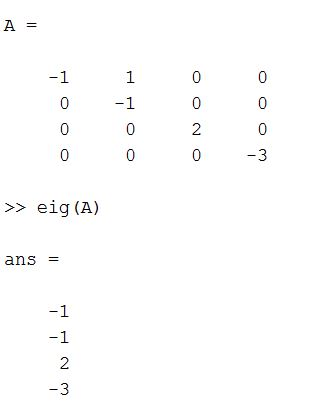
\includegraphics{6a}}
\end{center}

In order to find the zeros of the of the system we will examine the corresponding transfer function of the system found for part b.\\ 
\\
(b) Corresponding transfer function\\
Using MATLAB the corresponding transfer function for the system is found to be
\begin{align*}
\begin{bmatrix}
\frac{2s+4}{s^2+4s+3} && 0\\\frac{1}{s^2+2s+1} && \frac{1}{s+1}
\end{bmatrix}
\end{align*}
From the above transfer function the zeros of the system can be found by calculating the zeros of the determinant.  The determinant of the above function is 
\begin{align*}
\frac{4}{(1+s)(3+4s+s^2)}+\frac{2s}{(1+s)(3+4s+s^2)}
\end{align*}
Setting s=-2, the determinant is zero.  Therefore, we can say that the zero of the system is -2.\\
\\
(c) Stability\\
For stability analysis, there are several ways that we can determine if the system is stable or not.  One such way is to look at the transfer function, and if each entry in G(s) has poles in the open left half plane, the system is said to be BIBO stable.  The transfer function above, tells us that all entries contain poles in the open left half plane except the entry which is 0.  This would lead us to believe that the system is in fact BIBO stable.  Also, see hand written pages for integral method to determine stability.\\
\\ 
(d) Controllability and Observability\\
In order to examine the controllability of a state-space system, the controllability matrix must be calculated.  The controllability matrix is given by:

\begin{align*}
C(A,B)=\begin{bmatrix}B && AB && A^2B && A^3B\end{bmatrix}
\end{align*}

Mathematica will be utilized to calculate the controllability matrix.\\
From Mathematica, we find that the controllability matrix is

\begin{align*}
\begin{Bmatrix}\begin{bmatrix}0 && 1\\1 && 0\\0 && 0\\1 && 0\end{bmatrix}&& \begin{bmatrix}1 && -1\\-1 && 0\\0 && 0\\-3 && 0\end{bmatrix} && \begin{bmatrix} 1 && 1\\1 && 0\\0 && 0\\9 && 0\end{bmatrix} && \begin{bmatrix}1 && -1\\-1 && 0\\0 && 0\\-27 && 0\end{bmatrix}
\end{Bmatrix}
\end{align*}

A row of zeros can be seen in the Controllability matrix, which means that the system is rank deficient, and in turn not controllable. We can also say that the rank of the controllability matrix is 4.  In order to determine which state is uncontrollable, we need to calculate a few more matrices.  By observation, we expect that the uncontrollable state is $x_3$, and we will prove this in the following way:

\begin{align*}
\lambda I-A=\begin{bmatrix} \lambda+1 && -1 && 0 && 0\\0 && \lambda+1 && 0 && 0\\0 && 0 && \lambda-2 && 0\\0 && 0 && 0 && \lambda+3\end{bmatrix}\\
\begin{bmatrix}\lambda I-A && B_1\end{bmatrix}=\begin{bmatrix} \lambda+1 && -1 && 0 && 0 && 0\\0 && \lambda+1 && 0 && 0 && 1\\0 && 0 && \lambda-2 && 0 && 0\\0 && 0 && 0 && \lambda+3 && 1\end{bmatrix}
\end{align*}

plugging in $\lambda=-1$ the controllability matrix becomes:

\begin{align*}
\begin{bmatrix}\lambda I-A && B_1\end{bmatrix}=\begin{bmatrix} 0 && -1 && 0 && 0 && 0\\0 && 0 && 0 && 0 && 1\\0 && 0 && -3 && 0 && 0\\0 && 0 && 0 && 2 && 1\end{bmatrix}
\end{align*}

The rank for the above matrix is equal to the rank of the Controllability Matrix,4, meaning that the first and second states are controllable by the first input. Now we compute a similar matrix using $B_2$\\

\begin{align*}
\begin{bmatrix}\lambda I-A && B_2\end{bmatrix}=\begin{bmatrix} \lambda+1 && -1 && 0 && 0 && 1\\0 && \lambda+1 && 0 && 0 && 0\\0 && 0 && \lambda-2 && 0 && 0\\0 && 0 && 0 && \lambda+3 && 0\end{bmatrix}
\end{align*}
Again, we let $\lambda=-1$ and compute the rank of the resulting matrix

\begin{align*}
\begin{bmatrix}\lambda I-A && B_2\end{bmatrix}=\begin{bmatrix} 0 && -1 && 0 && 0 && 1\\0 && 0 && 0 && 0 && 0\\0 && 0 && -3 && 0 && 0\\0 && 0 && 0 && 2 && 0\end{bmatrix}
\end{align*}

The rank of the resulting matrix is less than the rank of the Controllability Matrix, meaning that the state with a pole at $\lambda=-1$ is not controllable by the second input.  In order to get a full description of which states are controllable through which inputs, the process above would be continued for each eigenvalue and for each input.  Since the initial observation led us to think that the third state was the uncontrollable state, I will skip the intermediate steps and compute the matrices that will tell us about the controllability of the state of interest by the input of interest.\\

We will examine $\lambda=2$ for both instances of the controllability matrix.

\begin{align*}
\begin{bmatrix}\lambda I-A && B_1\end{bmatrix}=\begin{bmatrix} 3 && -1 && 0 && 0 && 0\\0 && 3 && 0 && 0 && 1\\0 && 0 && 0 && 0 && 0\\0 && 0 && 0 && 5 && 1\end{bmatrix}
\\
\begin{bmatrix}\lambda I-A && B_2\end{bmatrix}=\begin{bmatrix} 3 && -1 && 0 && 0 && 1\\0 && 3 && 0 && 0 && 0\\0 && 0 && 0 && 0 && 0\\0 && 0 && 0 && 5 && 0\end{bmatrix}
\end{align*}
For both cases above, the rank of the resulting matrix is rank deficient (rank=3), telling us that the third state is not controllable by either input.  We will further conclude (from inspection) that states $x_1$ is controllable by input $u_1$, state $x_2$ is controllable by inputs $u_2$ and $u_1$, and state $x_4$ is controllable by input $u_2$.\\
\\
Now the subject of Observability must be analyzed.  In this case, an Observability matrix will be calculated which is defined to be:

\begin{align*}
O(A,C)=\begin{bmatrix}C\\CA\\CA^2\\CA^3\end{bmatrix}
\end{align*}

Using Mathematica the following result was found.

\begin{align*}
O(A,C)=\begin{bmatrix}0 && 1 && 0 && 1\\1 && 0 && 0 && 0\\0 && -1 && 0 && -3\\-1 && 1 && 0 && 0\\0 && 1 && 0 && 9\\1 && 1 && 0 && 0\\0 && -1 && 0 && -27\\-1 && 1 && 0 && 0\end{bmatrix}
\end{align*}

The above matrix has rank equal to 3, due to a column of zeros in the third column.  To determine the states that are not observable, we compute the following matrices to observe their rank and compare it to the rank of the Observability matrix.

\begin{align*}
\begin{bmatrix} \lambda I-A \\ C_1 \end{bmatrix}=\begin{bmatrix} \lambda+1 && -1 && 0 && 0\\0 && \lambda+1 && 0 && 0\\0 && 0 && \lambda-2 && 0\\0 && 0 && 0 && \lambda+3\\ 0 && 1 && 0 && 1 \end{bmatrix}
\\
\begin{bmatrix}\lambda I-A \\ C_2 \end{bmatrix}=\begin{bmatrix} \lambda+1 && -1 && 0 && 0\\0 && \lambda+1 && 0 && 0\\0 && 0 && \lambda-2 && 0\\0 && 0 && 0 && \lambda+3\\ 1 && 0 && 0 && 0 \end{bmatrix}
\end{align*}  

Just as the specific states were compared to the specific inputs in the Controllability matrices, I will go through the same process for the Observability.\\
Setting $\lambda=-1$, we get the following matrices

\begin{align*}
\begin{bmatrix} \lambda I-A \\ C_1 \end{bmatrix}=\begin{bmatrix} 0 && -1 && 0 && 0\\0 && 0 && 0 && 0\\0 && 0 && -3 && 0\\0 && 0 && 0 && 2\\ 0 && 1 && 0 && 1 \end{bmatrix}
\\
\begin{bmatrix}\lambda I-A \\ C_2 \end{bmatrix}=\begin{bmatrix} 0 && -1 && 0 && 0\\0 && 0 && 0 && 0\\0 && 0 && -3 && 0\\0 && 0 && 0 && 2\\ 1 && 0 && 0 && 0 \end{bmatrix}
\end{align*}  

The rank of the first matrix is 3 and the second is 4. From our initial observation, we would expect the first state to be observable through the second output which would mean that the rank of the matrix of interest would have to be equal to the rank of the observability matrix in order to be observable.  Abiding strictly by the rules, this information tells us that the first state is observable through the second output.  For the sake of saving trees, I will jump to the analysis of $x_3$ to determine its observability, for this I will set $\lambda=2$.\\

\begin{align*}
\begin{bmatrix} \lambda I-A \\ C_1 \end{bmatrix}=\begin{bmatrix} 3 && -1 && 0 && 0\\0 && 3 && 0 && 0\\0 && 0 && 0 && 0\\0 && 0 && 0 && 5\\ 0 && 1 && 0 && 1 \end{bmatrix}
\\
\begin{bmatrix}\lambda I-A \\ C_2 \end{bmatrix}=\begin{bmatrix} 3 && -1 && 0 && 0\\0 && 3 && 0 && 0\\0 && 0 && 0 && 0\\0 && 0 && 0 && 5\\ 1 && 0 && 0 && 0 \end{bmatrix}
\end{align*}  
\\
The rank of the above matrices is 3.  Since the rank of the observability matrix is 3, this leads us to the conclusion that $x_3$ is observable through both outputs.  In fact, this should not be the case (from initial observation), and one would think that $x_3$ should not be observable.\\
\\
(e) Signals that appear in the output when the input is zero and initial state is nonzero\\
\\
To get an idea of what the output of the system would look like given zero input and a nonzero initial state, I simulated the system using MATLAB and looked at its response to nonzero initial conditions.  The image shown below is a response to initial conditions given by
\begin{center} 
$x0=\begin{bmatrix}1 && 1 && 1 && 1\end{bmatrix}$\\
{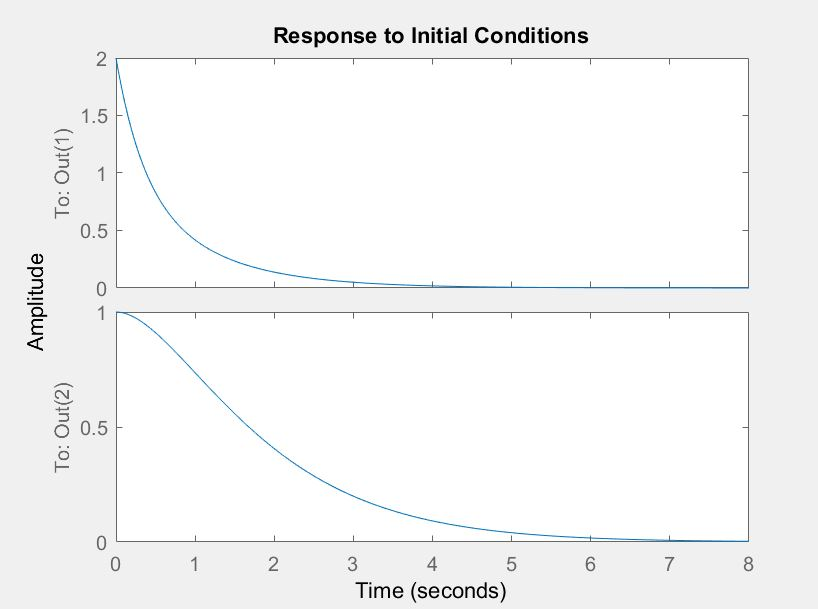
\includegraphics{6e}}
\end{center}
(f) Signals that appear in the state when the input is zero and initial state is nonzero\\ 
For this instance, the transfer function of the system was used to build a block diagram in Simulink, with initial conditions equal to 1.  The state behaviors can be seen in the graph below:
\begin{center}
{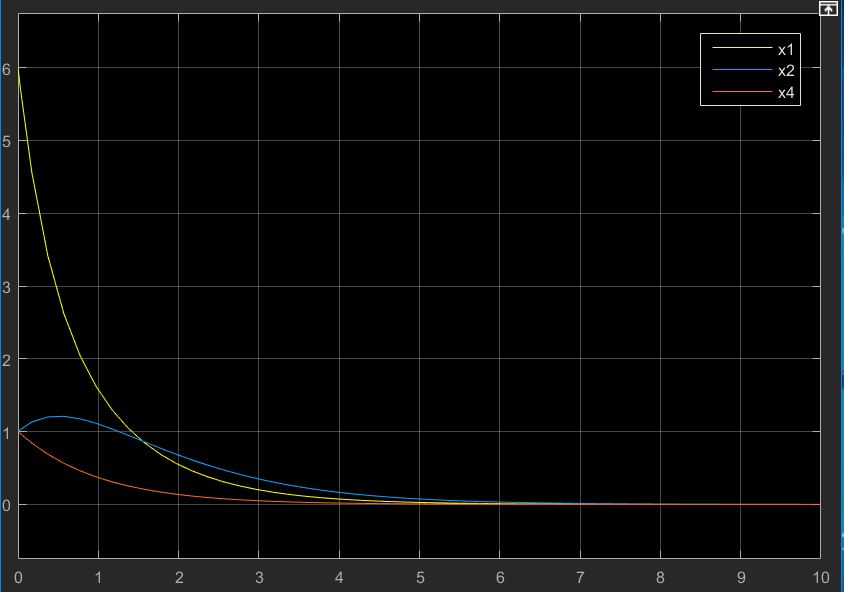
\includegraphics{6f}}
\end{center}
x3 is not shown on the graph because the state is unobservable.\\

(g) Minimal realization\\
\\
To get the minimal realization, I first start with the Observability Matrix defined in part (d).
\begin{align*}
O(A,C)=\begin{bmatrix}0 && 1 && 0 && 1\\1 && 0 && 0 && 0\\0 && -1 && 0 && -3\\-1 && 1 && 0 && 0\\0 && 1 && 0 && 9\\1 && 1 && 0 && 0\\0 && -1 && 0 && -27\\-1 && 1 && 0 && 0\end{bmatrix}
\end{align*}
From the matrix above, I need to take out the observable parts. For this exercise I will use the all powerful Mathematica to row reduce the Observability matrix to find the linearly independent rows (shown below).
\begin{center}
{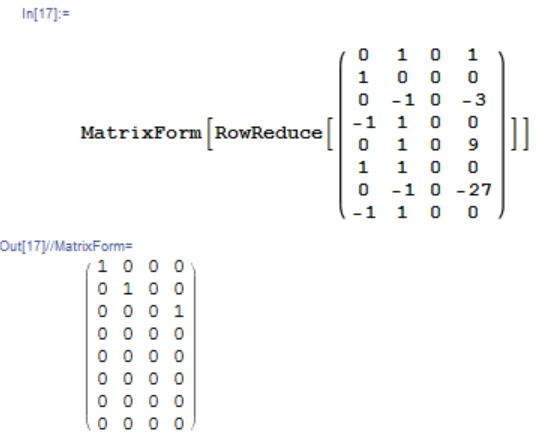
\includegraphics{6g}}
\end{center}
Now I see that the top three rows are the linearly independent rows which will be used to compose the matrix V
\begin{align*}
V^{-1}=\begin{bmatrix}V_1^T\\V_2^T\\V_3^T\\V_4^T\end{bmatrix}=\begin{bmatrix}0 && 1 && 0 && 1\\1 && 0 && 0 && 0\\0 && -1 && 0 && -3\\0 && 0 && 0 && 1\end{bmatrix}
\end{align*}
I continue along the minimal realization path by computing the following matrices
\begin{align*}
\bar{A}&=V^{-1}AV\\
\bar{B}&=V^{-1}B\\
\bar{C}&=CV\\
\end{align*}
\begin{center}
{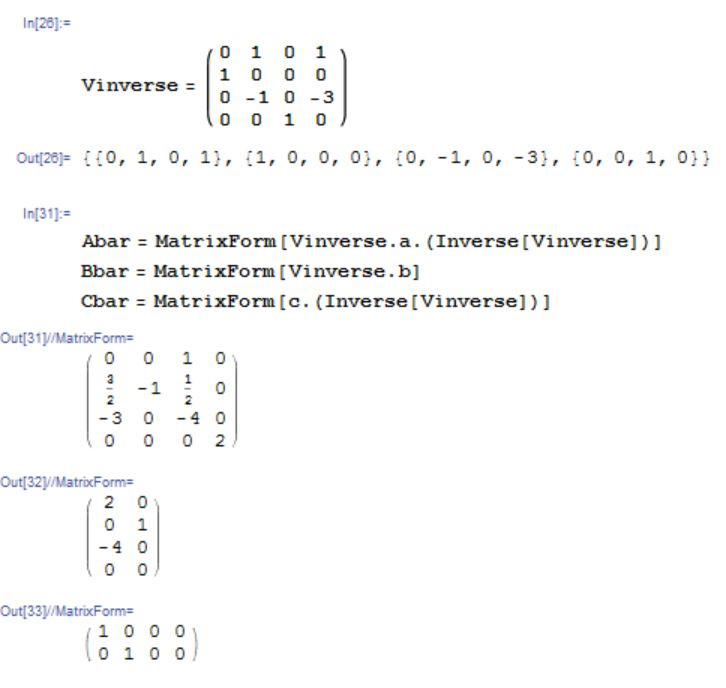
\includegraphics{6g2}}
\end{center}
The above figure shows the minimal realization (along with an arbitrary row) for the system of interest. 
\begin{align*}
A_m&=\begin{bmatrix}0 && 0 && 1\\ 3/2 && -1 && 1/2\\-3 && 0 && -4\end{bmatrix}\\
B_m&=\begin{bmatrix}2 && 0\\0 && 1\\-4 && 0\end{bmatrix}\\
C_m&=\begin{bmatrix}1 && 0 && 0\\0 && 1 && 0\end{bmatrix}
\end{align*}
The above system is the minimal realization!\\
(h) Anything else I can think of...\\
The graph describing the states given nonzero initial conditions looks very similar to the Blausias Similarity Solution for flat plate boundary layer flow (Shown Below).
\begin{center}
	{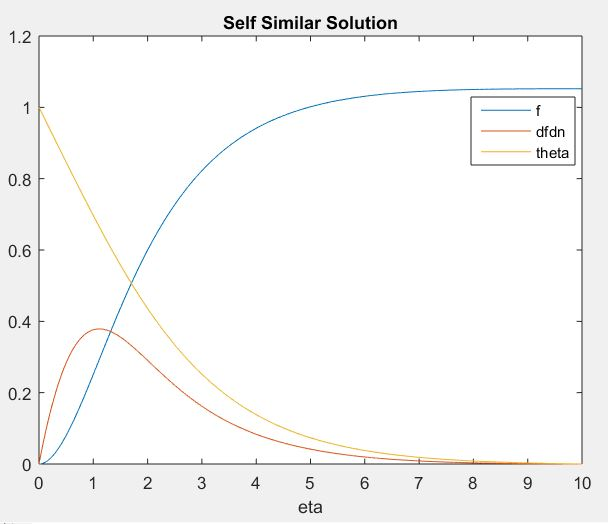
\includegraphics{Blasius}}
\end{center} 
Given a different set of boundary conditions the Blasius graph could resemble the states behavior identically.\\ 

\section*{Problem 7 (15 points)}
The circuit shown below has a voltage source, two capacitors, an inductor, and a resistor with the values shown.  The equations relating the system variables are:
\begin{align*}
u=i_1+v_1\\
i_2=0.25\frac{dv_2}{dt}\\
(i_1-i_2)=0.5\frac{dv_1}{dt}\\
v_1-v_2=0.333\frac{di_2}{dt}
\end{align*}
(a) Without writing any equations, discuss the proper number of states that should be used to describe the system.\\
\\
All electric components in the circuit are unique (i.e. there are no two capacitors, resistors or inductors that are the same), making it possible to back calculate a voltage or current at any point given voltage or current at another.  For this reason, I believe the proper number of states needed in order to describe the system is two. However, the minimal realization may tell us that we only need one state to fully describe the system and all other values can be back calculated using circuits laws.\\
\\
(b) Select appropriate variables to be the system states and write the state equations for the system, considering the input to be u and the output to be $y=v_2$.\\
\\
Defining the states to be:
\begin{align*}
x_1=v_1 && \dot{x_1}=\frac{dv_1}{dt}\\
x_2=i_2 && \dot{x_2}=\frac{di_2}{dt}
\end{align*}
The resulting equations become:
\begin{align*}
x_1&=\frac{1}{2}u\\
0.333\dot{x_2}-0.5\dot{x_1}&=0.25\dot{y}-y\\
\end{align*}

\end{document}